\chapter{Methods}

\section{Requirement Analysis}
  At the beginning of my work, I needed to assess the suitability of several possible targets at the RKI for NLP.
  Therefore, if applicable, I monitored the functioning of the target groups and evaluated their used textual sources.
  The direction of the thesis was determined based on the exploitability of the sources and the gain for the work practices through NLP.

  Below, I introduce available targets, and why they were or were not suitable for the proceedings of this thesis.

\subsection{RASFF}
  The Rapid Alert System for Food and Feed (\GLS{RASFF}) has been established by the European Union (\GLS{EU}) to share information for effective food safety.
  As a member of the RASFF, the RKI receives PDFs about recent incidences of contaminated food.
  Such a PDF contains several prototypical information about the contamination.

  However, the document is strongly formatted, and my attempts to extract the text from the PDF without altering the structure of the report failed.
  I used Tika (\ref{Tika}) for the text extraction, but the return contained misplaced line breaks and other formatting errors.
  Due to these complications and difficulties to extract text from these PDFs without optical character recognition, I decided not to consider the RASFF reports for my thesis.

\subsection{EpiLag}
  Due to the majority of communication in the EpiLag happening orally and the sources mainly being reports from medical practices, hospitals, and emails, EpiLag poses an ambitious target for NLP methodology.
  Without a clear in- and output, there is no clear approach to process the data of EpiLag.

\subsection{EPIS}
  As the RASFF, the Epidemic Intelligence Information System (\GLS{EPIS}) is also an EU project.
  It is a web tool that allows several EU members to report alarming disease outbreaks.
  To stay up-to-date, EPIS has an email notification system, and every outbreak report is downloadable as a formatted Excel sheet.

  The downside of EPIS is a missing source for reported outbreaks.
  Mostly, local health departments detect these events which are then shared through EPIS leaving out how they were discovered.
  This procedure makes the comparison of events difficult especially since different countries might not share the same definition for a disease outbreak.
  Though the formatted data output of EPIS would have been ideal for my further work, the regulations on how to process EPIS data were unclear and partially restrictive which excluded to further work with EPIS data.

\subsection{INIG}\label{INIGsources}
  The INIG has a curated list of sources that they visit every day and check for new alerting events (Tab. \ref{table:INIGsources}).
  The list consists of a various set of sources where some are frequently reporting and some less but in more extent.
  Also, the data format is different and can be a simple HTML website, PDF, or email.
  The rather easy and public access to the used sources, the clearly defined in- and output, and necessary active acquisition of information as described in EBS makes INIG a good fit for my topic.

\section{Libraries}
  In the following sections, I am introducing the most important libraries I used for my work.
  The list lacks libraries that are common for data-driven work with Python or are part of the standard library.

\subsection{NLTK}
  The Natural Language Tool Kit (\GLS{NLTK}) is an established and large package for NLP.
  It has 50 corpora and lexical resources as well as all important algorithms to build an NLP-pipeline as in Fig. \ref{fig:pipeline}.
  NLTK was built initially to teach NLP and thus, contains also outdated algorithms in the field of NLP.

  I used the stop word list, and the word and sentence tokenizer provided by NLTK.
  Furthermore, I used the multinomial NBC in NLTK to investigate the features with the highest explanatory power for classification, i.e., words that influence the classification decision by NBC the most.

\subsection{EpiTator}
  EpiTator is an epidemiological annotation library that is mainly used by \href{https://grits.eha.io}{GRITS}.
  I used the following features of EpiTator in my thesis:
  \begin{itemize}
    \item EpiTator's count annotator that extracts the glyph and word representation for numbers and associated attributes, e.g., \textit{``5 cases of smallpox''} will detect \textit{5} as a count and \textit{cases} as its attribute
    \item The date annotator that extracts dates and date ranges from a text
    \item EpiTator's geoname annotator that extracts all geographical entities from a text.
    \item Finally, I also used Epitator's resolved keyword annotator, that uses an SQLite database of entities to detect disease entities from multiple synonyms of infectious.
  \end{itemize}

\subsection{SpaCy}
  SpaCy is an industrial NLP library that contains every basic algorithm as illustrated in \ref{fig:pipeline}, but also newer methods from the field of deep learning such as CNNs and word embeddings.
  Additionally, SpaCy is written in the much fast CPython language.
  Altogether, speed and a selection of only the best-performing algorithms for NLP tasks give SpaCy the industrial strength.

  I used SpaCy's text classification module which uses a simple CNN.
  SpaCy is also mainly used by EpiTator for preprocessing.
  Also, saving the output of EpiTator was difficult because SpaCy is not trivial to serialize.
  Therefore, I needed to transform the output of EpiTator such that it did not contain SpaCy dependencies anymore.

\subsection{Flair}
  Flair is a small library that only contains state-of-the-art algorithms in NLP.
  It does not directly provide preprocessing such as stop word removal, tokenization, or stemming but does the preprocessing automatically depending on the final task.

  Flair has a powerful word embedding module that offers to stack different embeddings which I used for the text classification pipeline.

\subsection{Beautiful Soup}
  Beautiful Soup is a package to parse HTML and XML as a tree structure that can be traversed.
  Given the structured access to HTML content via tags, classes or ids, web scraping is much simpler with Beautiful Soup.
  I performed web scraping solely with Beautiful Soup.

\subsection{Boilerpipe}
  Boilerpipe is a Java package that uses shallow text features (word count, hyperlink density, and position of text block) to remove \emph{boilerplate} (advertisement, navigation bars,\dots) from websites \citep{Kohlschutter2010}.
  There exists a Python package that calls the Boilerpipe Java code from a Python environment.

  Although it was possible to have written the web scrapers such that they would have only extracted the main content, I wanted to have a solution that allows expanding the work of my thesis to more websites without the necessity to write a special scraping program for each site.
  Thus, I wrote scrapers that extract the whole HTML content of a site containing some outbreak article and then used Boilerpipe to obtain the main purport.

\subsection{Apache Tika}\label{Tika}
  Apache Tika is a broad content analysis framework for text and metadata extraction from over a thousand data types that I used for text extraction from PDFs.

\subsection{Luigi}
  Luigi is a pipeline builder made by Spotify.
  It manages different jobs, coordinates dependencies, and visualizes them.
  It is similar to GNU Make but offers more flexibility for data-heavy tasks or task scheduling.

  With Luigi, I modularize my work in case there is a requirement to modify or replace certain parts of my pipeline and automatically serialize the outcome of long and tedious computations such as scraping.

% \subsection{Sacred}
  Sacred helps to track experiments by saving the hyper-parameters, model name, and performance of those experiments, e.g., a machine learning model which I used to track my results.

\subsection{Flask}
  Flask is a web development mini-framework for Python.
  To demonstrate the final product which is capable of extracting the main content from some URL, annotating the key information of this content and then putting this information into a database, I built a web app using Flask.

\section{Data Acquisition}
  After the decision was made to focus on data associated with INIG, I pinpointed the most important sources (described in \ref{edb analysis}) used by INIG to build a labeled dataset.
  In the following, I show the necessary data required for the labeling, building, and preprocessing of the dataset.

\subsection{Incident Database - \textit{Ereignisdatenbank}}
  The \textbf{Ereignisdatenbank} (\GLS{EDB}) is an Excel sheet and the primary recording method of the work of INIG.
  They track various parts of their work in this sheet but most importantly they enter every critical outbreak article into the EDB.
  Every entry consists of several columns, of which only some are mandatory such as the reported \textbf{disease}, the \textbf{country} of origin, the number of \textbf{confirmed cases}, and the case number's reporting \textbf{date}.
  All WHO DON or ProMED Mail articles and the corresponding key information placed in the mandatory columns of these articles function as the training examples for the later mentioned classification algorithms.

\subsection{WHO DONs}
  The WHO regularly publishes the latest disease outbreak news (DONs) as a publicly available web resource.
  It is a low output source with only a handful of reports every week.
  All WHO DONs are archived, sorted by year and month, and therefore can be systematically accessed.

  I wrote a scraper that accesses the archive URL and then, based on the function parameter, visits the URL with the requested time range and scrapes the content (Lis. \ref{lst:who}).

  \begin{listing}[h]
    \begin{minted}[autogobble]{python}
      # Obtain annual report archive links
      page = requests.get('http://www.who.int/csr/don/archive/year/en/')
      soup = BeautifulSoup(page.content, 'html.parser')
      archive_years = soup.find('ul', attrs={'class': 'list'})
      all_years_links = archive_years.find_all('a')
      years_as_links = ['http://www.who.int' + link.get('href')
                        for link in all_years_links]

      # Obtain all report URLs per year
      for year_link in years_as_links:
        page_year = requests.get(year_link)
        soup_year = BeautifulSoup(page_year.content, 'html.parser')
        archive_year = soup_year.find('ul', attrs={'class': 'auto_archive'})
        daily_links = ['http://www.who.int' + link.get('href')
                       for link in  archive_year.find_all('a')]
    \end{minted}
    \caption{An extract from the WHO DONs scraping script. The algorithm starts with extracting the content of \textquotesingle \texttt{http://www.who.int/csr/don/archive/year/en}\textquotesingle, then filters the URLs for those referencing archived reports of all years with the help of the \texttt{ul} tag and \texttt{list} class. To extract all DONs per year, the \texttt{auto\char`_archive} class is used. All links are found in the \texttt{a} tag and \texttt{href} selector.}
    \label{lst:who}
  \end{listing}

\subsection{ProMED Mail}
  Opposed to WHO DONs, much more authors are contributing to ProMED Mail and therefore generate higher output.
  Usually, ProMED publishes around a handful of disease outbreak articles a day.
  ProMED mail content is dynamically loaded via Ajax and therefore not directly accessible.
  Through the analysis of the website, I reverse engineered the article search of the website to write a function with which I can scrape ProMED article given a time range shown in Lis. \ref{lst:promed}.
  Access to the page number shown in Lis. \ref{lst:promed} is necessary since after 200 pages the GET request returns an error although there would be more pages.
  The full algorithm iterates over 200 pages given a time range, remembers the date of the oldest ProMED article from this search and reruns the search with the initial temporal lower bound and the date of the last retrieved article as the newer upper bound.

  \begin{listing}[h!]
    \begin{minted}[autogobble]{python}
    def get_content_of_search_page(from_date, to_date, page_num):
      return (requests
              .get(f'https://www.promedmail.org/ajax/runSearch.php?'
                   f'pagenum={page_num}&'
                   f'search=&date1={from_date}&'
                   f'date2={to_date}'
                   )
              .content
              .decode('utf-8')
              )
    \end{minted}
    \caption{The ProMED scraping core function. It executes a formatted Ajax GET request (indicated as a string in the \texttt{requests.get} method) for a certain date range and page number which returns a list of ProMED article URLs in the form of \textquotesingle \texttt{https://www.promedmail.org/direct.php?id=6400233}\textquotesingle. Everything in curly brackets is replaced by the function parameters.}
    \label{lst:promed}
  \end{listing}

\subsection{Wikipedia - Liste der Staaten der Erde}\label{wikipedia}
  I scraped the \href{https://de.wikipedia.org/wiki/Liste_der_Staaten_der_Erde}{Wikipedia Liste der Staaten der Erde} (\textit{List of Sovereign States}) article and transformed it into a dictionary to translate the German country names of the EDB into English.
  The translation is an crucial step to match the countries in the EDB with the output of EpiTator to automatically create a labeled dataset \ref{edb analysis}.
  The List of Sovereign States contains, besides others, the state's common, formal, and English name, and also the ISO-2 and ISO-3 abbreviation.
  The code for scraping the table from the Wikipedia page is shown in Lis. \ref{lst:wikipedia}

  \begin{listing}[h]
    \begin{minted}[autogobble]{python}
      # Request the HTML content from Wikipedia and parse it with BeautifulSoup
      req = requests.get("https://de.wikipedia.org/wiki/Liste_der_Staaten_der_Erde")
      soup = BeautifulSoup(req.content, "html.parser")

      # Find table with all countries with HTML tag "table",
      # the CSS class "wikitable sortable zebra", and the "tbody" tag
      table_soup = soup.find("table", class_="wikitable sortable zebra")
      body_soup = table_soup.find("tbody")

      # Get entries of all countries form table
      country_soup = body_soup.find_all("tr")
    \end{minted}
    \caption{Python code extract to scrape the Liste der Staaten der Erde table from Wikipedia using BeautifulSoup. The table is extracted using the \texttt{table, tbody} and \texttt{tr} tag and the \texttt{wikitable sortable zebra} class.}
    \label{lst:wikipedia}
  \end{listing}

\subsection{Wikidata and RKI-Internal Data}\label{wikidata}
  I queried all disease names in German and English from \href{https://www.wikidata.org/wiki/Wikidata:Main_Page}{Wikidata} (Lis. \ref{lst:wikidata}) and used them as a dictionary to transform all German disease names of the EDB to English to be able to match them with EpiTator's output to create a labeled dataset (\ref{edb analysis}).
  Additionally, I used a list of RKI-internal abbreviation to translate them to their full English name.

  \begin{listing}[h]
    \begin{minted}[autogobble]{python}
      endpoint_url = "https://query.wikidata.org/sparql"
      query = """SELECT Distinct ?itemLabel_DE   ?itemLabel_EN WHERE {
                  ?item wdt:P31 wd:Q12136.
                  OPTIONAL{
                  ?item rdfs:label ?itemLabel_DE.
                  FILTER (lang(?itemLabel_DE) = "de"). }
                  ?item rdfs:label ?itemLabel_EN.
                  FILTER (lang(?itemLabel_EN) = "en").
                  }"""
      disease_translation_dictonary = get_results_of_sparql(endpoint_url, query)
    \end{minted}
    \caption{The SPARQL request made to retrieve a list of tuples with the German and English disease name from Wikidata where \texttt{wdt:P31 wd:Q12136} is the item name of the disease list in Wikidata.}
    \label{lst:wikidata}
  \end{listing}

\section{Preprocessing}
  The EDB is an unstructured Excel sheet which means that the data types were not restricted, no uniform vocabulary was used, and formatting errors occurred several times.
  The EDB needed to be machine-parsable and be comparable with the output of EpiTator (\ref{edb analysis}) to assign positive labels to the output of EpiTator if it matches the corresponding entries from the mandatory columns of the EDB.
  After the description of the EDB, and the scraping of dictionaries to transform EDB entries into English, I show the necessary steps to clean the EDB, make it machine-readable, and transform it into a controlled English vocabulary to be comparable with the output of EpiTator.

\subsection{Variables}
  The EDB has many entries where only a handful is mandatory.
  During the preprocessing, I only kept the mandatory entries.
  The \textbf{URL} of the article, the \textbf{disease}, the \textbf{country} of outbreak as mentioned in the article, and the \textbf{confirmed case count} with the \textbf{date} as of the date count are used for further processing.

  The preprocessing steps were the removal of empty rows, trailing white spaces, and the split-up of several entries in one cell to several rows or the merge of redundant columns to be per the tidy data concept \citep{Wickham2014}.
  The crucial part of the preprocessing was, however, the transformation of the variables into a controlled vocabulary.

\subsection{Controlled Vocabulary}\label{controlled vocabulary}
  \paragraph{Dates}
    The dates needed to be transformed into a pandas Timestamp object on which arithmetic operations and comparison are possible.
    This was done with the \texttt{pandas.totimestamp()} method.
    If the method is provided with the information whether date or month is mentioned first, \texttt{pandas.totimestamp()} automatically recognizes several forms of dates and transfers them into the correct Timestamp object.

  \paragraph{Counts}
    Every case count entry in the EDB was cleaned from any non-digit entry.
    In the case of several numerical values, the first one was taken.

  \paragraph{URLs}
    I removed invalid URLs, and transformed ProMED URLs into a uniform style. The ProMED URLs in the EDB are written with both, \texttt{http} and \texttt{https} as a protocol. Furthermore, ProMED URLs in the EDB are written like \textquotesingle \texttt{https://\allowbreak www.promedmail.org\allowbreak /post\allowbreak /6400233} \textquotesingle as an example or without the \texttt{www.} preceding the URL. However, to be consistent with the scraped URL format returned by Lis. \ref{lst:promed}, I transformed all URLs into the form \textquotesingle \texttt{https://\allowbreak www.promedmail.org/\allowbreak direct.php?id=6400233} \textquotesingle.

  \paragraph{Countries and diseases}
    Country and disease names needed to be translated to make them comparable to the output of EpiTator.
    Therefore, I used the scraped dictionaries as in \ref{wikidata}, \ref{wikipedia} through which I eradicated spelling mistakes and translated these words to English.
    The procedure is shown in Algo. \ref{lst:translate}.
    %
    \begin{algorithm}[h]
    \SetAlgoLined
      \KwIn{$t_{\neg controlled}$}
      \KwResult{$t_{controlled}$}
      \tcc{Initialize}
      $\operatorname{dictionary}: K_{\neg controlled} \to V_{controlled}$\;
      \uIf{$t_{\neg controlled} \in K$}{
        \Return $\operatorname{dictionary}(t_{\neg controlled})$\;
        }
        \Else{
        \[ \operatorname{lev}_{a,b}(i,j) = \begin{cases}
        \max(i,j) \hfill \text{ if } \min(i,j)=0, \\
        \min \begin{cases}
          \operatorname{lev}_{a,b}(i-1,j) + 1 \\
          \operatorname{lev}_{a,b}(i,j-1) + 1 \\
          \operatorname{lev}_{a,b}(i-1,j-1) + 1_{(a_i \neq b_j)}
       \end{cases} \hfill \text{ otherwise.}
       \end{cases}\]
       \tcc{Where lev is the Levenshtein distance of word $a$ and $b$ at string $i$ of $a$ and $j$ ob $b$.}
       $t_{corrected} \leftarrow \argmin_{k \in K} \operatorname{lev}_{\neg controlled, k}$\;
         \uIf{$t_{corrected} \in K$}{
            \Return $\operatorname{dictionary}(t_{corrected})$\;
            }
        \Else{$t_{corrected} \leftarrow \operatorname{endsOrStartsWith}(t_{\neg controlled}, dictionary)$\;
        \Return $\operatorname{dictionary}(t_{corrected})$\;}
        }
      \caption{Translation algorithm to transform input to controlled vocabulary. If initially no translation is available, the most similar written word is chosen using the the Levenshtein distance. The word $k \in K$ with the shortest Levenshtein distance to the input word $t_{\neg controlled}$ is picked to correct the input word. If there is still no match to the controlled vocabulary, the algorithm assumes a shortened form and searches for an overlap in the first or last letters of the strings.}
      \label{lst:translate}
      \end{algorithm}

\subsection{NLP-Pipeline}
  The WHO DONs and the ProMED Mail articles needed to be prepared for the ML algorithms.
  In the following, I describe the steps of the NLP-pipeline each text underwent before being fed into a classification algorithm.

\subsubsection{Literal Processing}
  In the case of PDFs, I replaced unrecognized characters, indicated by the Unicode code \texttt{U+FFFD}, by one single white space.
  In the case of the scraped HTML, I replaced all UTF-8 control characters with a single whitespace characters illustrated by the following Python code: \mintinline[breaklines]{python}{string = "".join(char if unicodedata.category(char)[0] != "C" else ' ' for char in string)}.

\subsubsection{Embedding}
  I used Flair to apply pretrained GloVe embeddings with 50 dimensions on each token of the dataset.

\section{Classification}
  I trained a classifier to be able to distinguish between \textsl{relevant} and \textsl{irrelevant} outbreak news based on the whole text, and based on the embeddings of the text.

  Furthermore, I tested two methods for the key information extraction: First, taking the most frequent entity occurring in a text as the key entity (e.g., making the most common disease entity as the primary thematized in the text) and second, train a classifier based on sentences that contain such entities.
  The training data were all sentences-tokenized ProMED and WHO DON articles of 2018.
  Sentences containing the keywords found in the corresponding EDB entry are the positive training labels.
  All other sentences containing keyword entities of the same category (e.g., confirmed cases) recognized by EpiTator, but are not found in the respective EDB entry, are counterexamples for the classifier.

  The full pipeline of all steps necessary before the assembly of the labeled training dataset are depicted in Fig. \ref{fig:dataset}

  \begin{figure}[h!]
    \centering
    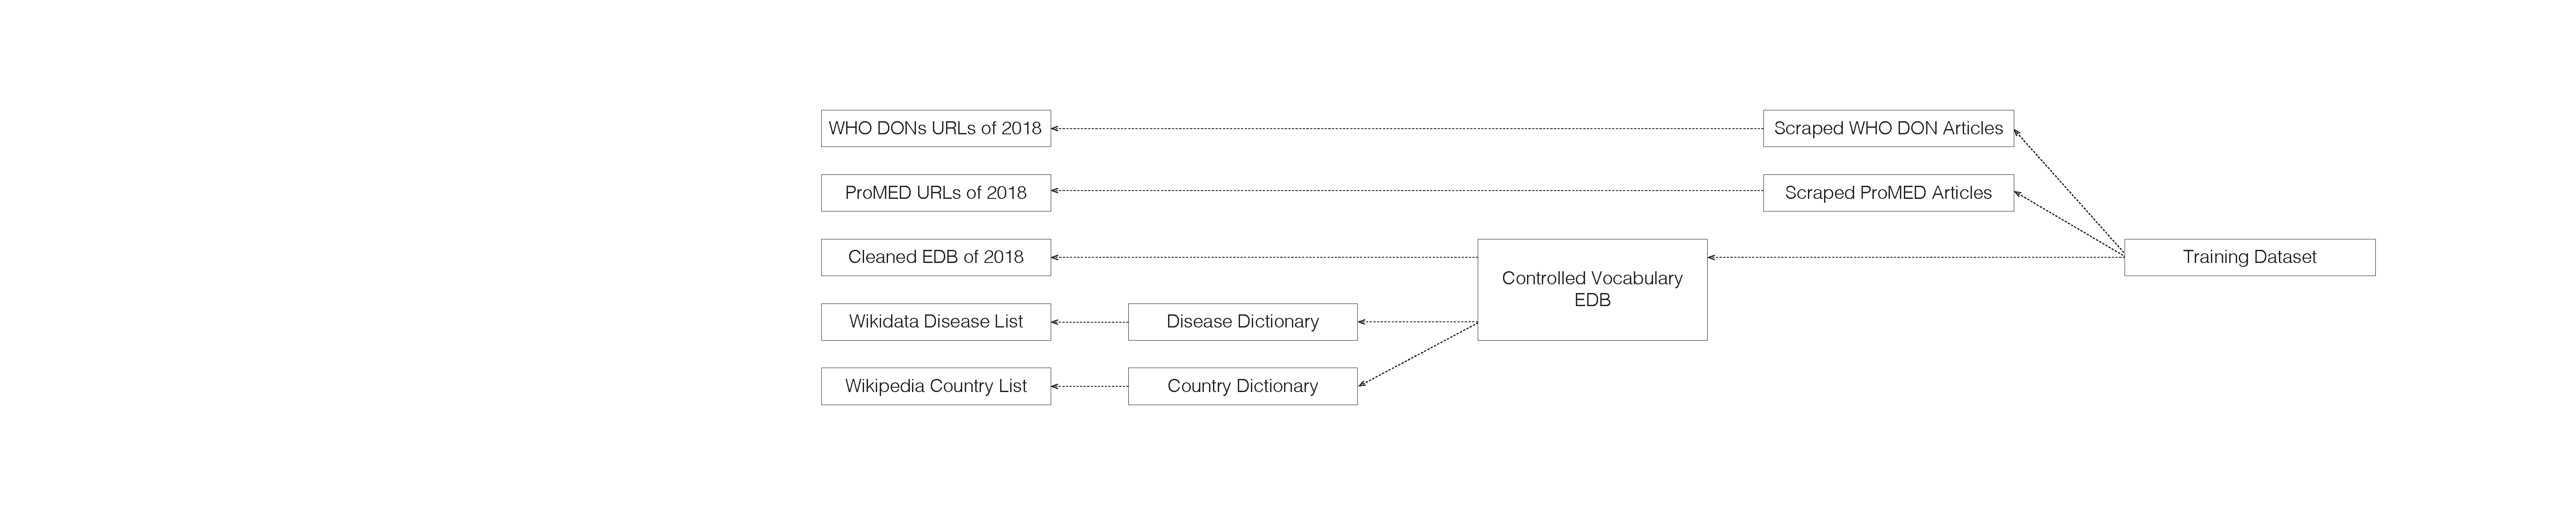
\includegraphics[scale=0.25]{dataset.pdf}
    \caption{A depiction of all the dependencies during the assembly of the labeled dataset.}
    \label{fig:dataset}
  \end{figure}


\subsection{Naive Key Word Extraction}
  During the reading of epidemiological news, I noticed that the key entities of a text are repeatedly mentioned.
  Therefore, I decided to naively determine a keyword entity by choosing the most occurring entity, i.e., the key disease entity would be the disease mentioned most frequently as shown in Lis. \ref{lst:mostoccure}.
  \begin{listing}[h!]
    \begin{minted}[autogobble, breaklines]{python}
      def return_most_occuring_entities(list_of_entities):
        list_of_entity_occurence_tuple = [(key, len(list(group)))
                                          for key, group
                                          in groupby(sorted(list_of_strings))]
        most_occuring_string = max(list_of_entity_occurence_tuple,
                                   key=itemgetter(1))[0]
        return most_occuring_string
    \end{minted}
    \caption{A simplified Python function to detect the most occurring entity in a list of entities.}
    \label{lst:mostoccure}
  \end{listing}

\subsection{Naive Bayes Classifier}\label{iskey}
  I used the multinomial and complement NBC for the text classification using all WHO DONs and ProMED Mail articles of the year 2018.
  Articles denoted in the EDB are labeled \textsl{relevant} and the rest is labeled \textsl{irrelevant}.
  I applied tf-idf to balance term frequency discrepancies.

  For the keyword extraction, I used the multinomial and Bernoulli NBC for each entity class fed by all sentences containing this entity class.
  Sentences of texts that contain entities found in the corresponding EDB entity entry for this text are labeled as \textsl{is key} whereas the rest is labeled \textsl{is not key}.

\subsection{Deep Learning}
  For a visualization of the available corpus, I self-trained word embeddings using word2vec with the continuous bag-of-words model approach.
  During the text classification, I first used the average of all word embeddings as the document embedding and fed it into a multilayer perceptron with 100 neurons in the hidden layer, a rectified linear unit as the activation function, the Adam optimizer using the default values during training, and L2 penalty to avoid overfitting.
  Also, I used a CNN to iterate over all word embeddings using an automatically selected feature map size by SpaCy, and average pooling.
  For the classifier trained on embeddings, I used ADASYN to upsample the dataset.

\section{Web App}
  Using Flask and \href{https://www.datatables.net}{DataTables}, I built a web app that allows the entry of an URL where then the text is extracted, summarized, and put into a data table which can be downloaded in various formats.
  The web app also contains a method to start an automatic scraping of all articles from a specified source up to the last analyzed article from this source. These texts are then annotated and dumped it into the database.
